\section{Euklidinen taso. Geometriset luvut} \label{geomluvut}
\alku
\sectionmark{Euklidinen taso}

Oletetaan lähtökohtaisesti tutuiksi sellaiset geometrian käsitteet kuin
\begin{itemize}
\item  \kor{piste}, \kor{suora}, \kor{jana} 
\item  \kor{kulma}, \kor{kolmio}, \kor{$n$-kulmio}, \kor{monikulmio}, \kor{yhdenmuotoisuus}
\item  \kor{suunta} (\kor{puolisuora}, säde), \kor{yhdensuuntaisuus}, \kor{suunnikas}
\item  \kor{suora kulma}, \kor{Pythagoraan lause}, \kor{suorakulmio}
\item  \kor{ympyrä}, janan \kor{pituusmitta} ('mittatikku')
\end{itemize}
Näiden taustalla ovat euklidisessa geometriassa lähtökohtana oletetut perusaksioomat, jotka 
tunnetaan \kor{Hilbertin aksioomina}\footnote[2]{Saksalainen \hist{David Hilbert} (1862-1943)
oli modernin matematiikan suunnannäyttäjä ja kaikkien aikojen huomattavimpia matemaatikkoja. 
Hilbert tunnetaan mm.\ hänen v. 1900 asettamistaan ratkaisemattomista matematiikan ongelmista, 
jotka sittemmin on nimetty \kor{Hilbertin ongelmiksi}. Euklidisen geometrian perusaksioomat ovat
peräisin Hilbertin pienestä klassikkoteoksesta ''Grundlagen der Geometrie'' vuodelta 1899. Teos
oli ensimmäinen kattava ja systemaattinen esitys geometrian --- myös eräiden epäeuklidisten 
geometrioiden ---  aksiomaattisista perusteista.}.

Euklidisen tason perusolioita ovat p\pain{isteet}, joista muiden olioiden (kuten jana, suora 
ym.) ajatellaan koostuvan. Euklidista tasoa sanotaankin \kor{pisteavaruudeksi}. Sen symbolinen
merkki on \Ekaksi, luetaan 'E kaksi'.
\vspace{5mm}
\begin{figure}[htb]
\begin{center}
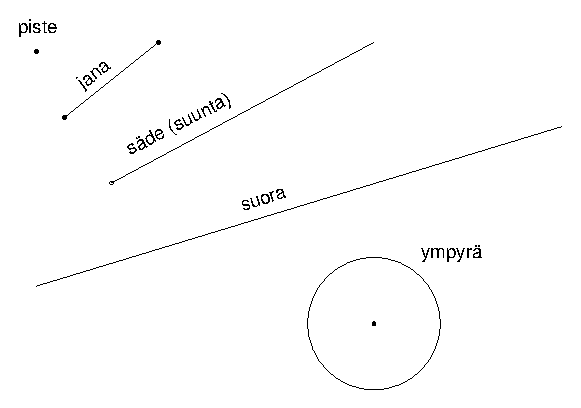
\epsfig{file=kuvat/kuvaII-1.eps}
\end{center}
%\caption{Euklidisen tason olioita}
\label{fig:oliot}
\end{figure}

Huomattakoon, että euklidisessa geometriassa \pain{ei} lähtökohtaisesti oleteta esim.\ 
sellaisia käsitteitä kuin
\begin{itemize}
\item  kulman mitta ('astelevy'), ympyräkaaren pituus, ympyräsektorin pinta-ala
\end{itemize}
Sen sijaan voidaan haluttaessa olettaa
\begin{itemize}
\item  (suorakulmaisen) \kor{kolmion pinta-ala} ('mittasisältö')
\item  pinta-alan \kor{additiivisuus} (= yhteenlaskettavuus) monikulmiossa
\end{itemize}

Sellaiset geometriset operaatiot kuin yhdensuuntaisten suorien piirtäminen, suoran kulman
konstruoiminen, tai annetun geometrisen olion (pistejoukon) \kor{siirto} ja \kor{kierto}
eli nk.\ \kor{euklidinen} \kor{liike} (esim.\ janan siirtely pituus säilyttäen) tapahtuvat
euklidisessa geometriassa ympyräviivojen (käytännössä harpin) avulla. Myös suora on 
konstruoitavissa pelkästään harppia käyttäen, sillä suora on sellaisten pisteiden joukko
eli \kor{ura}, jotka ovat yhtä etäällä kahdesta annetusta pisteestä. --- Viivoitinta 
tarvitaan geometriassa siis vain pisteiden 'massatuotantovälineenä'. 

\kor{Kulman} määrittelee geometriassa kaksi suuntaa. Konkreettisemmin ajatellaan kulma
yleensä pistejoukoksi, jonka muodostavat kaksi samasta pisteestä lähtevää
puolisuoraa.\footnote[2]{Kulma voidaan myös tulkita puolisuorien rajaamaksi euklidisen
tason \kor{sektoriksi}, jolloin on tehtävä ero \kor{sisäkulman} ja \kor{ulkokulman} välillä.}
Näin ymmärrettynä kaksi kulmaa ovat \kor{yhtä suuret} ('samat'),
jos ne voidaan muuntaa toisikseen euklidisella liikkeellä.\footnote[3]{Kulmien
yhtäsuuruus on kulmien joukossa määritelty ekvivalenssirelaatio, vrt.\ Luku \ref{logiikka}.} 
Jos kahden kolmion (vastin)kulmat ovat yhtä suuret, niin kolmiot ovat \kor{yhdenmuotoiset}.
Jos myös (vastin)sivujen pituudet ovat samat, kolmiot ovat \kor{yhtenevät}. Tällöin ne
voidaan muuntaa toisikseen joko euklidisella liikkeellä tai yhdistämällä euklidiseen
liikkeeseen \kor{peilaus} (suoran suhteen).

Todistettaessa geometrisia väittämiä alkuperäisen geometrian keinoin vedotaan usein
y\pain{hdenmuotoisuuso}p\pain{in} (geometrian aksioomista seuraavaan) väittämään:
Yhdenmuotoisissa kolmioissa vastinsivujen pituuksien suhteet ovat samat 
(vrt.\ Harj.teht.\,\ref{H-II-1: yhdenmuotoisuus}). 

Käsiteltäessä kulmia geometrisina olioina (harpin avulla) voidaan määrätä geometrisesti
myös kahden kulman \kor{summa} ja \kor{erotus} tukeutumatta kulmien mittalukuihin.
Operaatiot tapahtuvat siirtelemällä kulmia euklidisella liikkeellä niin, että ne joutuvat
joko 'vierekkäin' (summa) tai 'päällekkäin' (erotus). Geometrisella yhteenlaskulla on
esimerkiksi todennettavissa tunnettu kolmion kulmia koskeva väittämä: Kulmien summa = 
\kor{oikokulma} (Harj.teht.\,\ref{H-II-1: kulmat}).

\subsection*{Geometriset luvut}

Janan pituuden mittaus, työvölineenä harppi, tuo geometriaan reaaliluvut 
(tai ainakin osan niistä) ja myös lukuihin liittyvät laskutoimitukset. Lähtökohtana
pidetään lukuja $0$ ja $1$:
\[
0\ \vast\ \text{piste}, \quad 1\ \vast\ \text{mittajana}
\]
Kun tarkastellaan kiinteää suoraa, jolta valitaan referenssipiste $O$ luvun $0$ vastineeksi, 
niin kahden (janan pituutena) annetun luvun summa ja erotus voidaan määrätä geometrisesti:
\begin{figure}[htb]
\begin{center}
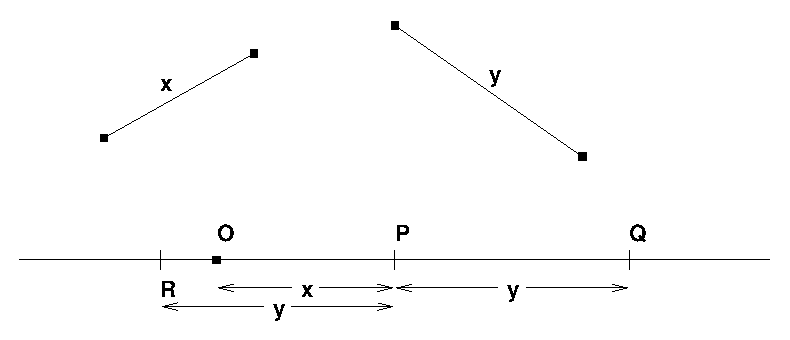
\epsfig{file=kuvat/kuvaII-2.eps}
\end{center}
%\caption{Kahden janan pituuksien summa ja erotus}
%\label{fig:summajaerotus}
\end{figure}

Kuvassa summalla ja erotuksella on geometriset vastineet janoina ja suoran pisteinä:
\begin{align*}
\qquad &x+y\ \vast\ OQ\ \vast Q  \\
\qquad &x-y\ \vast\ OR\ \vast R
\end{align*}
Kun janan loppupiste on $O$:sta vasemmalle (suuntahan oli määritelty!), voidaan $OR$ tulkita 
negatiiviseksi luvuksi $x-y$. Näin on siis lukujärjestelmässä määritelty sekä yhteenlasku että
vähennyslasku. Kun sääntöjä $+,-$ sovelletaan peräkkäin lähtien luvusta 1 (= mittajana
sijoitettuna suoralle) nähdään, että minkä tahansa kokonaisluvun $m\in{\Z}$ geometrinen vastine
saadaan äärellisellä määrällä geometrisia operaatioita. Siis {\Z} on konstruoitu geometrisesti.
Myös millä tahansa kokonaisluvulla jakaminen onnistuu 'siivuttamalla' luku yhdensuuntaisilla 
suorilla, joita voidaan \pain{tasossa} tuottaa harpilla ja viivoittimella (ks.\ kuvio alla).

Yleisemmin jos lähtökohtana on kaksi mittalukua $x,y$, niin niiden välinen kerto- ja jakolasku
voidaan suoraan geometrisoida yhdenmuotoisten kolmioiden avulla käyttäen suhteita 
\[
\frac{z}{x}\ =\ \frac{y}{1} \quad (z=xy) \qquad \text{ja} \qquad
\frac{z}{1}\ =\ \frac{x}{y} \quad (z=x/y)
\]
\begin{figure}[htb]
\begin{center}
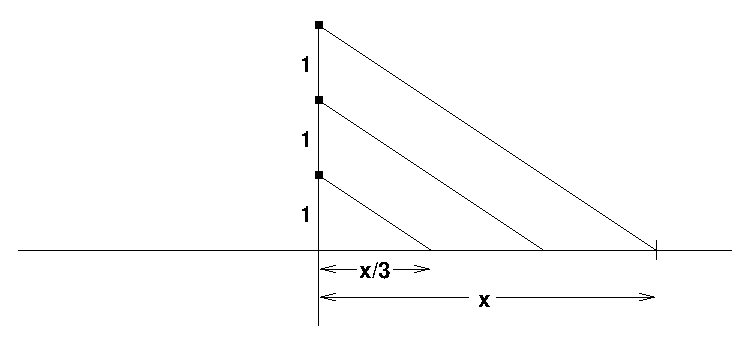
\epsfig{file=kuvat/kuvaII-3.eps}
\end{center}
\end{figure}
Kuvassa (alla) on
\begin{alignat*}{3}
OA &\ \vast\ 1,\quad & OB &\ \vast\ y,\quad & BC&\ \vast\ OD\ \vast\ x \\
OE &\ \vast\ x\cdot y,\quad & AF &\ \vast\ x/y &&
\end{alignat*} 
\begin{figure}[H]
\setlength{\unitlength}{0.67cm}
\begin{center}
\begin{picture}(12,9)(-3.5,-6)
\put(-2,0){\line(1,0){11}}
\put(-0.1,-0.1){$\bullet$} \put(-0.5,0.5){$O$}
\put(2.9,-0.1){$\bullet$} \put(3,-0.6){$A$}
\put(4.9,-0.1){$\bullet$} \put(4.9,-0.6){$B$}
\put(7.9,1.9){$\bullet$} \put(7.9,2.4){$C$}
\put(4.7,1.1){$\bullet$} \put(4.3,1.4){$F$}
\put(-1.84,-3.26){$\bullet$} \put(-1.5,-3.4){$D$}
\put(-3.02,-5.4){$\bullet$} \put(-2.6,-5.5){$E$}
\put(-3,-4){\line(3,2){11}}
\put(-3.5,-5.67){\line(3,2){12.5}}
\put(-2,-0.5){\line(4,1){11}}
\path(0,0)(-3.5,-6.34)
\put(0,-0.2){$\underbrace{\hspace{2cm}}_1$}
\put(0,0.4){$\overbrace{\hspace{3.33cm}}^y$}
\put(6.8,0.8){$x$}
\put(7.2,1.1){\vector(3,2){1.15}}
\put(6.55,0.7){\vector(-3,-2){1}}
\put(-1.3,-1.6){$x$}
\put(-1.1,-1.3){\line(10,18){0.6}}
\put(-0.5,-0.25){\vector(2,3){0.13}}
\put(-1.3,-1.8){\line(-10,-19){0.6}}
\put(-1.9,-2.92){\vector(-2,-3){0.05}}
\end{picture}
\end{center}
\end{figure}
Jatkossa nimetään luvut, jotka ovat konstruoitavissa (janan pituutena) äärellisellä määrällä
geometrisia operaatioita, \kor{geometrisiksi luvuiksi}\footnote[2]{Englanninkielinen termi on 
'constructible numbers'. Suomennos ei ole vakiintunut.}, ja käytetään tälle lukujoukolle 
symbolia $\G$\,:
\begin{align*}
\G \ = \ \text{\{geometriset luvut\}}
\end{align*}
Tiedetään jo, että $\G$ sisältää kaikki rationaaliluvut: $\G\supset\Q$. Lisäksi tiedetään, että
$\G$ on peruslaskutoimitusten suhteen suljettu:
\[
x,y \in \G \qimpl x+y,\ x-y,\ xy,\ x/y \in \G \quad (y\neq0)
\]
Tämä merkitsee, että $(\G,+,\cdot)$ on \pain{kunta}.

Lukujoukon $\G$ muodostamisessa eivät geometrian mahdollisuudet lopu aivan 
peruslaskutoimituksiin, sillä Pythagoraan lauseen mukaan myös operaatiot
\begin{align*}
&x,y\ \map\ \sqrt{x^{2}+y^{2}}, \quad x,y \in \G \\
&x,y\ \map\ \sqrt{x^{2}-y^{2}}, \quad x,y \in \G,\ x \geq y
\end{align*}
ovat geometrisesti toteutettavissa. Erityisesti on siis vuosituhansia päänvaivaa aiheuttanut
luku $\sqrt{2}$ geometristen lukujen joukossa:
\begin{figure}[H]
\setlength{\unitlength}{1cm}
\begin{center}
\begin{picture}(2.5,2.5)(-0.5,0)
\path(0,2)(0,0)(2,0)(0,2)
\put(0.8,-0.5){$1$} \put(-0.3,0.9){$1$} \put(0.9,1.1){$\sqrt{2}$}
\path(0.15,0)(0.15,0.15)(0,0.15)
\end{picture}
\end{center}
\end{figure}
Itse asiassa neliöjuurioperaatio $\,x\ \map\ \sqrt{x}\,$ on geometrisesti mahdollinen, olipa
mittaluku $x \in \G$ (ajatellaan $x \geq 0$) mikä tahansa:
\begin{figure}[H]
\setlength{\unitlength}{1cm}
\begin{center}
\begin{picture}(7,4.5)(0,-0.5)
\path(3,4)(0,0)(3,0)(3,4)(8.33,0)(3,0)
%\put(3,0){\arc{0.6}{-3.14}{-1.6} \linethickness{0.05cm} \put(-0.12,0.12){\picsquare}}
%\put(3,4){\arc{0.6}{0.8}{2.2} \linethickness{0.1cm} \put(0,-0.15){\picsquare}}
\path(2.85,0)(2.85,0.15)(3,0.15) %\path(2.82,3.76)(3,3.625)(3.18,3.865)
\path(2.91,3.88)(3,3.812)(3.09,3.932)
\put(0,-0.2){$\underbrace{\hspace{3cm}}_{1}$} \put(3,-0.2){$\underbrace{\hspace{5.33cm}}_{x}$}
\put(2.8,1.9){$\left. \begin{array}{c} \vspace{3.4cm} \end{array} \right\} 
                                                                    \scriptstyle{y=\sqrt{x}}$}
\end{picture}
\end{center}
\end{figure}
Tähän geometrian mahdollisuudet kuitenkin loppuvat, joten $\G$ koostuu kaikkiaan luvuista, jotka
on saatu mittaluvusta $1$ lähtien äärellisellä määrällä viittä eri operaatiota: 
$+$, $-$, $\cdot\,$, $/$ ja $\sqrt{ }\,$. Kun $\G$ vielä varustetaan geometrisella 
järjestysrelaatiolla (janojen pituuksien vertailu harpin avulla), niin tuloksena on pelkästään
geometrisiin operaatioihin perustuva järjestetty kunta $(\G,+,\cdot,<)$. Tämä on 
rationaalilukujen kunnan pienin mahdollinen laajennus, joka täyttää ehdon 
$x\in\G\,\ja\,x>0\ \impl\ \sqrt{x}\in\G$ (vrt.\ lukujoukon $\J$ konstruktio Luvussa \ref{kunta}).
On osoitettavissa, että kaikki geometriset luvut ovat algebrallisia (!), joten pätee
\[ 
\Q\ \subset\ \G\ \subset\ \A\ \subset\ \R.
\]
Kun geometriset luvut sijoitetaan em.\ tavalla kiinteälle suoralle, voidaan näiden lukujen 
'väliin' ajatella sijoitelluksi myös muut reaaliluvut. Näin ajatellen jokainen reaaliluku saa 
geometrisen vastineen \kor{lukusuoran} pisteenä.

\begin{figure}[H]
\setlength{\unitlength}{1cm}
\begin{center}
\begin{picture}(14,2)(-2,0)
\put(-1,0){\line(1,0){13}}
\put(0,0){\line(0,1){0.2}}
\put(5,0){\line(0,1){0.2}}
\put(10,0){\line(0,1){0.2}}
\put(20,0){\line(0,1){0.1}}
\put(2.07,0){\line(0,1){0.1}}
\put(8.6,0){\line(0,1){0.1}}
\put(10.7,0){\line(0,1){0.1}}
\put(2.07,1){\vector(0,-1){0.6}} \put(8.6,1){\vector(0,-1){0.6}} \put(10.7,1){\vector(0,-1){0.6}}
\put(-0.1,-0.5){$1$} \put(4.9,-0.5){$2$} \put(9.9,-0.5){$3$}
\put(1.8,1.5){$\sqrt{2}$} \put(8.5,1.5){$e$} \put(10.6,1.5){$\pi$} 
%\multiput(0,2)(0,10){2}{\line(-1,0){0.1}}
%\multiput(0,6.5)(0,1){2}{\line(-1,0){0.1}}
%\put(-0.6,8){\vector(1,-1){0.5}}
%\put(-0.6,6){\vector(1,1){0.5}}
\end{picture}
\end{center}
\end{figure}

\Harj
\begin{enumerate}

\item \label{H-II-1: kulmat}
Suoran leikatessa kaksi yhdensuuntaista suoraa syntyy neljä kulmaa. Päättele geometrisesti,
että kaikki neljä kulmaa ovat yhtä suuret, ja edelleen tähän nojaten: Kolmion kulmien summa
= oikokulma.

\item \label{H-II-1: yhdenmuotoisuus}
a) Jana jakaa suorakulmaisen kolmion kahteen osaan siten, että syntyy kolme yhdenmuotoista 
kolmiota. Lähtien tästä ajatuksesta ja kolmioiden yhdenmuotoisusopista todista Pythagoraan 
lause! \newline
b) Kolmion \kor{keskijana} yhdistää kolmion kärjen vastakkaisen sivun keskipisteeseen.
Lähtien kolmioiden yhdenmuotoisuusopista todista: Kolmion $ABC$ keskijana $AD$ puolittaa
jokaisen janan $BC$ suuntaisen janan, jonka päätepisteet ovat sivuilla $AB$ ja $AC$.

\item
Esitä geometrinen konstruktio (aseina harppi ja viivoitin), jonka tulos on \newline
a) \ ympyrä, joka kulkee annetun kolmen pisteen kautta, \newline
b) \ annetun kolmion sisään piirretty (suurin mahdollinen) ympyrä, \newline
c) \ suora, joka kulkee annetun pisteen kautta ja sivuaa (koskettaa yhdessä pisteessä)
annettua ympyrää.

\item
Mitkä seuraavista ovat geometrisia lukuja\,? \newline
a) \ $\sqrt[1024]{17}$ $\quad$ b) \ $\sqrt[3]{3}$ $\quad$ c) \ $\sqrt[6]{216}$ $\quad$
d) \ $\sqrt[3]{7\sqrt{2}+5}$ $\quad$ e) \ $\sqrt[3]{5\sqrt{2}+7}$

\item
Janalla $AB$ sijaitseva piste $C$ on janan \kor{kultainen leikkaus}, jos $a/b=b/c$,
missä $a,b,c$ ovat janojen $AB$, $AC$ ja $CB$ pituudet. Konstruoi $C$ geometrisesti
lähtien tunnetuista pisteistä $A$ ja $B$\,!

\end{enumerate}